\documentclass[aspectratio=169, table]{beamer}

%\usepackage[beamertheme=./praditatheme]{Pradita}
\usepackage[utf8]{inputenc}

\usetheme{Pradita}

\subtitle{MTI102-Information Systems \&\\Technology Architecture}

\title{TOGAF Framework and \\ Its Components}
\date[Serial]{\scriptsize {PRU/SPMI/FR-BM-18/0222}}
\author[Pradita]{\small {\textbf{Alfa Yohannis}}}

\begin{document}

    \frame{\titlepage}

    \begin{frame}
        \frametitle{What is the TOGAF Framework?}
        % \framesubtitle{\hspace{1cm}}
        \begin{itemize}
            \item TOGAF is a framework for enterprise architecture development.
            \item Developed by The Open Group, an IT industry consortium.
            \item Consists of methods and tools to assist in the design, implementation, and management of enterprise architecture.
            \item TOGAF focuses on architecture lifecycle management.
            \item Uses a repeatable and iterative life cycle approach.
        \end{itemize}
    \end{frame}

    \begin{frame}
        \frametitle{Architecture Domain}
        % \framesubtitle{\hspace{1cm}}
        \vspace{20pt}
        \begin{itemize}
            \item \textbf{Business Architecture}. Business strategy, governance, organisation and key business processes.

            \item \textbf{Data Architecture}. Organisational logical and physical data structures
            asset and resource data management.

            \item \textbf{Architecture Applications}. A blueprint for the individual application systems that will be deployed, their interactions, and their relationships to the organization's core business processes.

            \item \textbf{Architecture Technology}. Software and hardware capabilities required to support the deployment of business, data, and service applications. This includes IT infrastructure, middleware, networking, communications, processing, and standards.
        \end{itemize}
    \end{frame}

    {
        \setbeamertemplate{frametitle}{}
        \setbeamertemplate{navigation symbols}{}
        \setbeamertemplate{footline}{}
        \begin{frame}
            \frametitle{TOGAF Framework}
            \framesubtitle{\hspace{1cm}}
            \begin{center}
                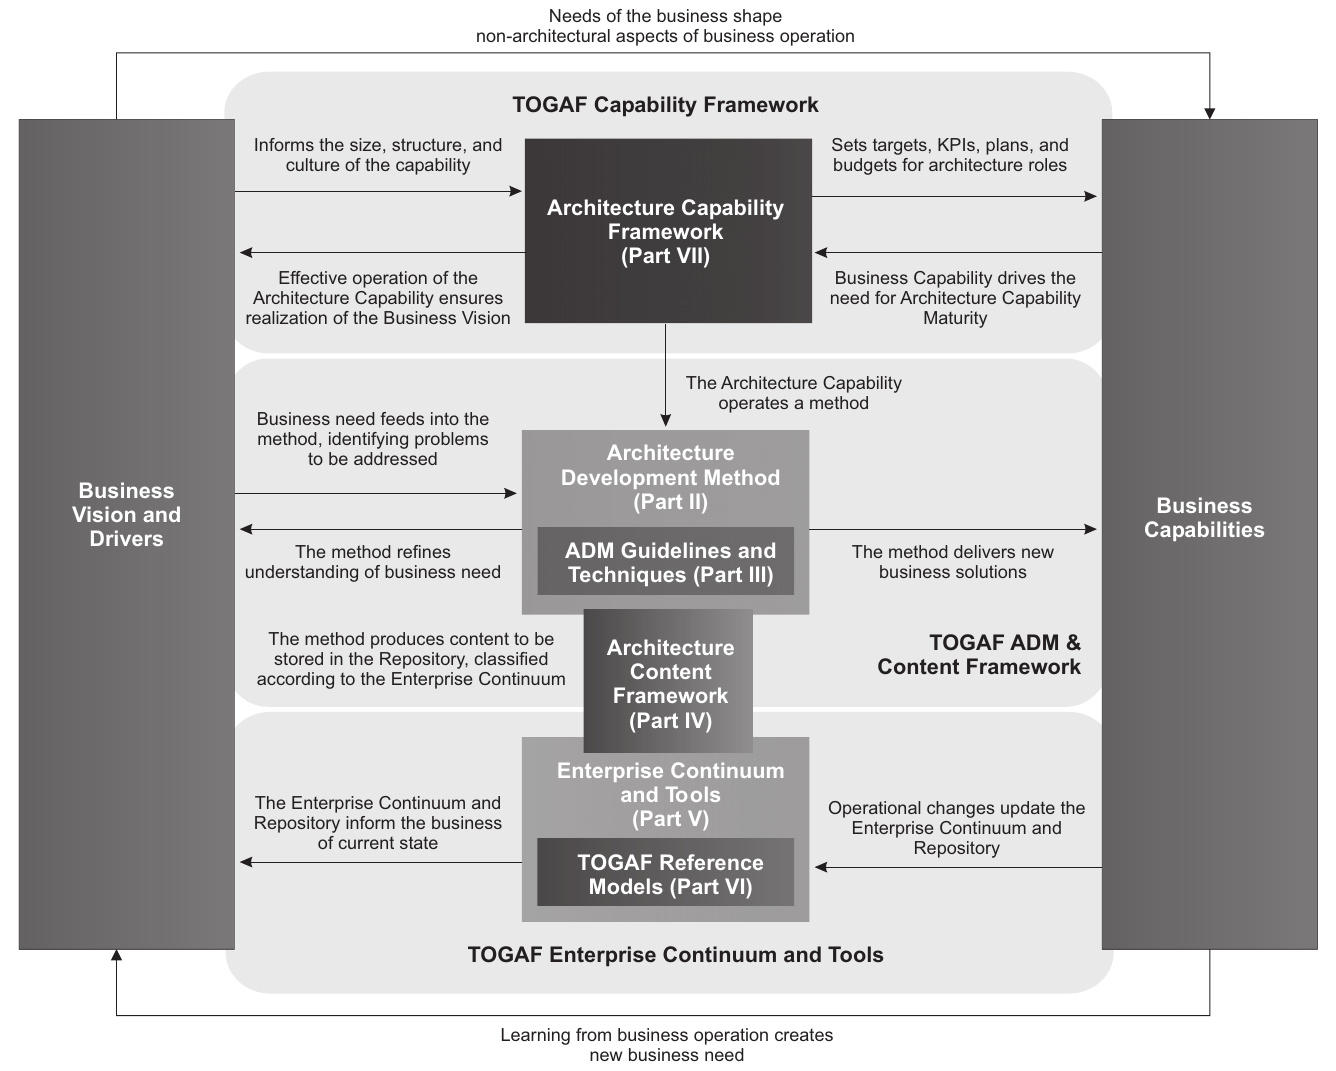
\includegraphics[width=.78\textwidth]{../figures/togaf}
            \end{center}
        \end{frame}
    }

    \begin{frame}
        \frametitle{TOGAF components}
        \framesubtitle{\hspace{1cm}}
        \begin{itemize}
            \item Business Visions and Drivers
            \item Business Capabilities
            \item Architecture Capability Framework
            \item Architecture Development Method
            \item ADM Guidelines and Techniques
        \end{itemize}
    \end{frame}

    \begin{frame}
        \frametitle{TOGAF components (2)}
        \framesubtitle{\hspace{1cm}}
        \begin{itemize}

            \item Architecture Governance Frameworks
            \item Architecture Content Framework
            \item Deliverables, Artifacts, and Building Blocks
            \item Enterprise Continuum and Tools
            \item Architecture Repository
            \item TOGAF Reference Models
        \end{itemize}
    \end{frame}

    \begin{frame}
        \frametitle{Vision and Business Drivers at TOGAF}
        % \framesubtitle{\hspace{1cm}}
        \begin{itemize}
            \item A business vision is a view of an organization's goals and future.
            \item Business drivers are factors that drive change in an organization.
            \item TOGAF uses business vision and drivers to help define enterprise architecture.
            \item The business vision and drivers are developed during the Preliminary and Architecture Vision phases of ADM.
            \item In TOGAF, business drivers can include factors such as technological changes, market changes, or regulatory changes.
        \end{itemize}
    \end{frame}

    \begin{frame}
        \frametitle{Business Capabilities in TOGAF}
        % \framesubtitle{\hspace{1cm}}
        \begin{itemize}
            \item Business capabilities are the combination of people, processes, and technology that enable an organization to achieve its goals.
            \item TOGAF views business capabilities as an integral part of the enterprise architecture.
            \item A good understanding of business capabilities can help in the design and implementation of effective architectures.
            \item Business capabilities are identified and defined during the ADM process.
            \item They are then used to assist in architectural design and implementation.
        \end{itemize}
    \end{frame}

    {
        \setbeamertemplate{frametitle}{}
        \setbeamertemplate{navigation symbols}{}
        \setbeamertemplate{footline}{}
        \begin{frame}
            \frametitle{Architecture Capability Framework}
            \framesubtitle{\hspace{1cm}}
            \begin{center}
                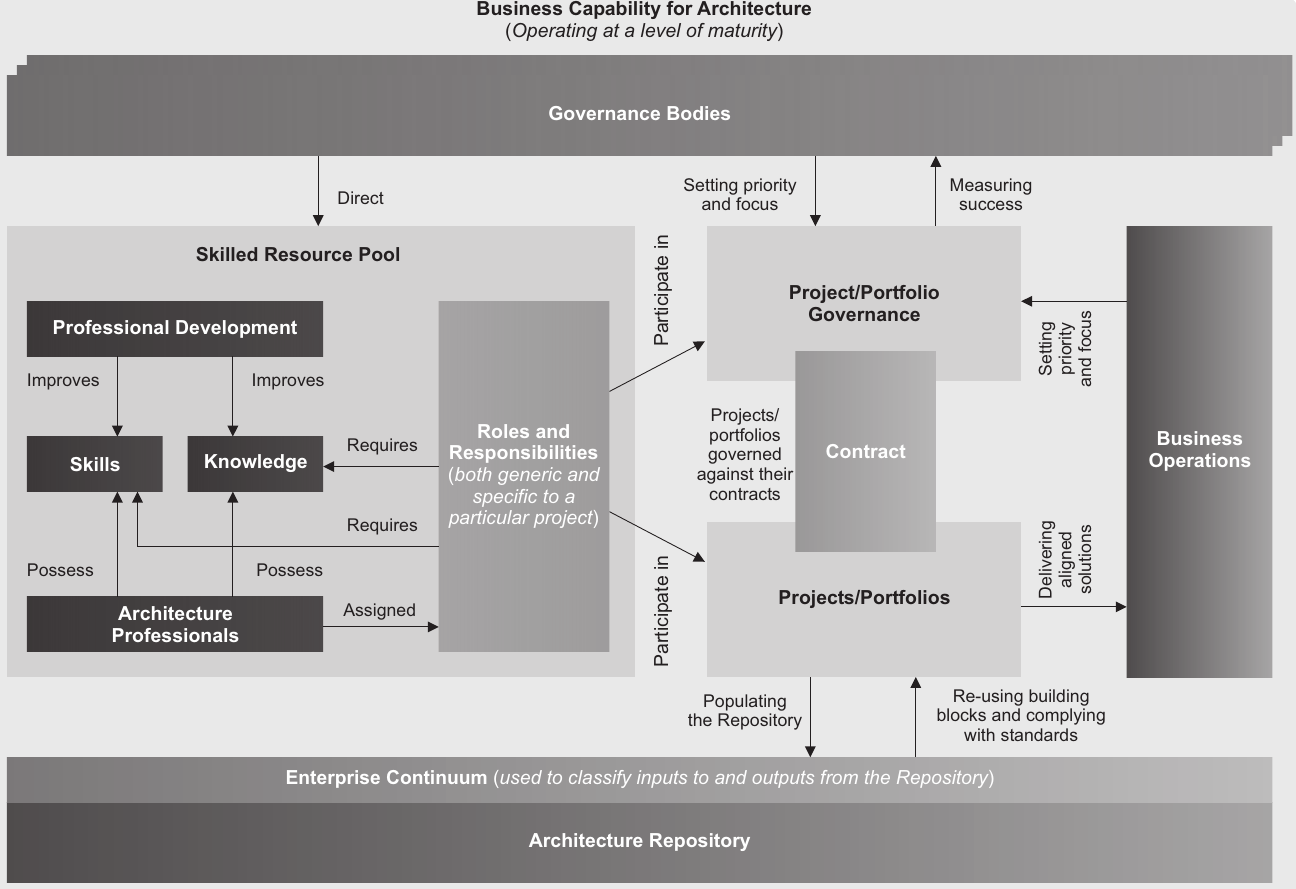
\includegraphics[width=.80\textwidth]{../figures/architecture_capability_framework}
            \end{center}
        \end{frame}
    }

    \begin{frame}
        \frametitle{TOGAF Architecture Capability Framework}
        \framesubtitle{\hspace{1cm}}
        \vspace{20pt}
        \begin{itemize}
            \item TOGAF 9 provides an Architecture Capability Framework which is a collection of reference materials and guidelines for building architectural functions
            or capabilities in the organization.
            \item Consists of seven categories: building architecture capabilities, architectural board, architecture compliance, architecture contracts, architecture governance, architecture maturity models, and architecture skills frameworks.
            \item Each category covers a set of capabilities necessary to produce an effective enterprise architecture.
            \item Using the Capability Framework, organizations can identify and close gaps in their capabilities.
        \end{itemize}
    \end{frame}

    \begin{frame}
        \frametitle{Contents of the TOGAF Architecture Capability Framework}
        \framesubtitle{\hspace{1cm}}
        \begin{enumerate}
            \item \textbf{Creating a Capability Architecture}. Setting up the necessary structures, processes, and roles to support the organization’s architecture practice (incl. scope, stakeholders, governance).
            \item \textbf{Architecture Board}. Overseer for the establishment and operation of the company's Architectural Council.
            \item \textbf{Architecture Compliance}.  Ensures that the organization’s architecture complies with relevant standards, policies, and regulations.
            \item \textbf{Architecture Contract}. Agreements that define define the scope, objectives, and deliverables.
        \end{enumerate}
    \end{frame}

    \begin{frame}
        \frametitle{Contents of the TOGAF Architecture Capability Framework (2)}
        \framesubtitle{\hspace{1cm}}
        \begin{enumerate}
            \setcounter{enumi}{4}
            \item \textbf{Architecture Governance}.  Ensures that the organisation’s architecture is aligned with business strategy and goals.
            \item \textbf{Architecture Maturity Model}. Help organisations assess the maturity of their architecture practice and identify areas for improvement.
            \item \textbf{Architecture Skills Framework}. A set of roles, skills, and experience norms for staff performing enterprise architecture work.
        \end{enumerate}
    \end{frame}


    \begin{frame}
        \frametitle{Architectural Development Method (ADM)}
        \framesubtitle{\hspace{1cm}}
        \vspace{20pt}
        \begin{itemize}
            \item ADM is the process recommended by TOGAF for developing enterprise architecture.
            \item Involves a series of organized phases that help in the design, planning, implementation, and management of enterprise architecture.
            \item These phases include Architectural Vision, Business Design, Information Design, Technology Design, to Implementation.
            \item ADM helps organizations manage the entire lifecycle of an enterprise architecture.
            \item ADM also provides guidelines and techniques for each phase of the development process.
        \end{itemize}
    \end{frame}

    {
        \setbeamertemplate{frametitle}{}
        \setbeamertemplate{navigation symbols}{}
        \setbeamertemplate{footline}{}
        \begin{frame}
            \frametitle{Architecture Development Method}
            \framesubtitle{\hspace{1cm}}
            \begin{center}
                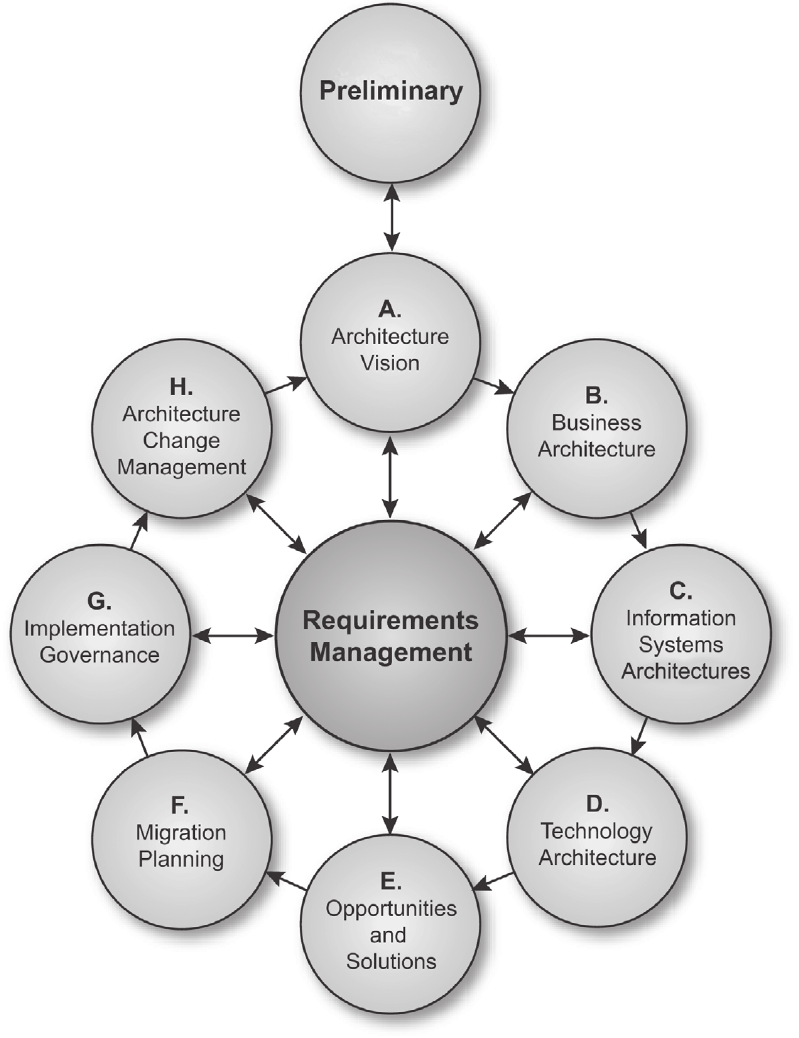
\includegraphics[width=.43\textwidth]{../figures/architecture_development_method}
            \end{center}
        \end{frame}
    }

    \begin{frame}
        \frametitle{ADM Guidelines and Techniques}
        % \framesubtitle{\hspace{1cm}}
        \begin{itemize}
            \item TOGAF provides a set of guidelines and techniques to assist in the implementation of ADM.
            \item This guidance helps organizations adapt ADM to their own needs and context.
            \item Some commonly used techniques include principles analysis, stakeholder analysis, gap analysis, business scenarios, migration plans, interoperability, risk management, capability plans.
        \end{itemize}
    \end{frame}

    \begin{frame}
        \frametitle{ADM Guidelines and Techniques (2)}
        % \framesubtitle{\hspace{1cm}}
        \begin{itemize}
            \item These guidelines and techniques ensure that the ADM process remains focused, efficient, and effective.
            \item Guidelines also help ensure that the resulting architecture aligns with business goals and objectives.
        \end{itemize}
    \end{frame}

    \begin{frame}
        \frametitle{Architecture Governance Framework }
        \framesubtitle{on TOGAF}
        \vspace{20pt}
        \begin{itemize}
            \item Architectural governance is the practice of managing and controlling an enterprise's architecture.
            \item In TOGAF, the architectural governance framework provides a structure for these practices.
            \item This framework includes aspects such as organizational structure, roles and responsibilities, processes, and communication methods.
            \item Architectural governance also involves creating and maintaining artifacts such as architectural principles, architectural models, and architectural roadmaps.
            \item The primary goal is to ensure that all projects remain aligned with the enterprise architecture and overall business strategy.
        \end{itemize}
    \end{frame}

    \begin{frame}
        \frametitle{Architectural Content Framework}
        % \framesubtitle{\hspace{1cm}}
        \begin{itemize}
            \item The Architectural Content Framework defines the types of architectural content required to cover the entire business domain.
            \item It guides the process of artifact identification, organization, and development.
            \item The Architecture Content Framework consists of three main components: Deliverables, Artifacts, and Building Blocks.
            \item Deliverables are the results of work provided to stakeholders. Artifacts are part of the Deliverables that describe the architecture.
            \item Building Blocks are the physical, logical, or conceptual components of a business or IT system.
        \end{itemize}
    \end{frame}



    \begin{frame}
        \frametitle{Deliverables, Artifacts, and Building Blocks in TOGAF}
        \framesubtitle{\hspace{1cm}}
        \begin{itemize}
            \item Deliverables are the results of architectural work provided to stakeholders.
            \item Artifacts are parts of Deliverables that describe the architecture in varying levels of detail.
            \item Building Blocks are the physical, logical, or conceptual components of a business or IT system.
            \item Examples of Deliverables: Architectural Vision Document, Migration Plan.
            \item Artifact Examples: Data Diagrams, Application Diagrams. Examples of Building Blocks: server, application, database.
        \end{itemize}
    \end{frame}

    {
        \setbeamertemplate{frametitle}{}
        \setbeamertemplate{navigation symbols}{}
        \setbeamertemplate{footline}{}
        \begin{frame}
            \frametitle{Architecture Deliverables}
            \framesubtitle{\hspace{1cm}}
            \begin{center}
                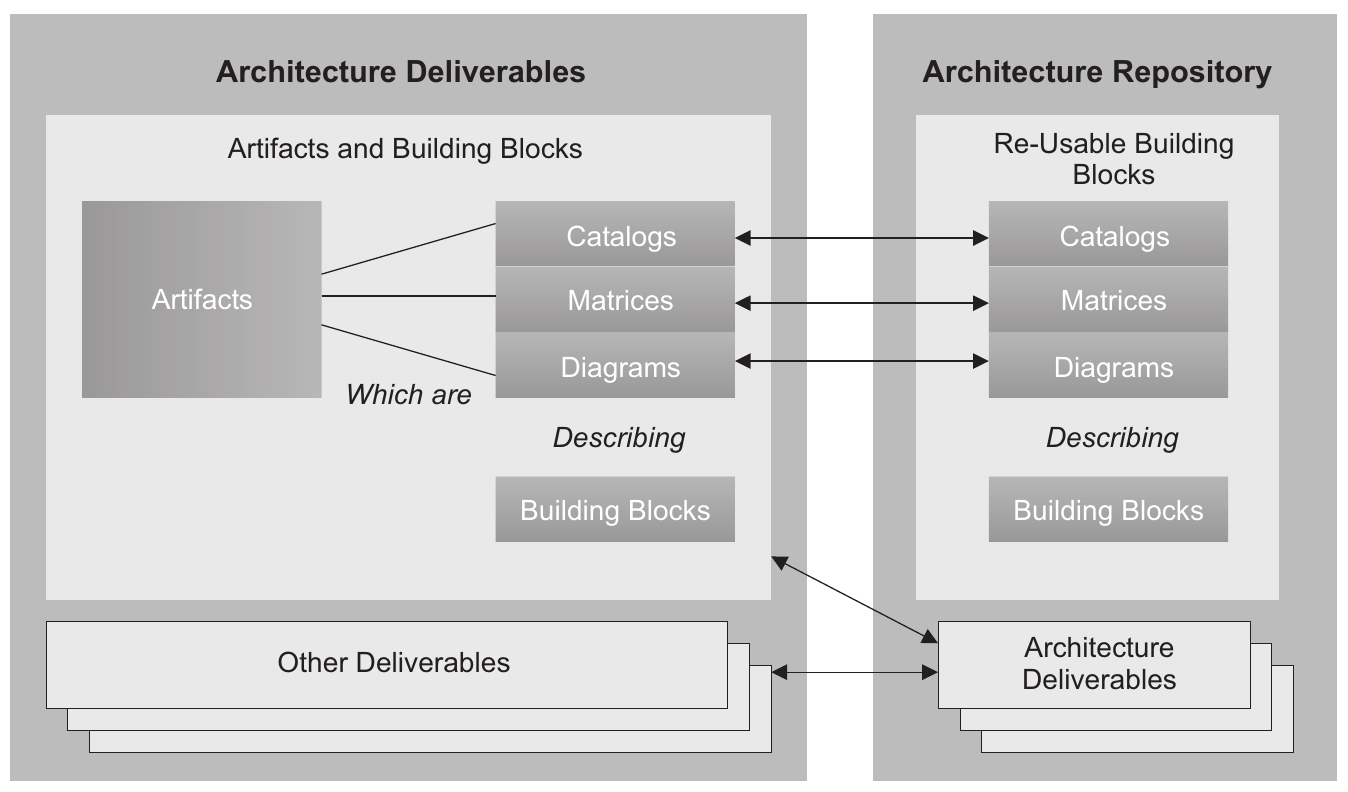
\includegraphics[width=.95\textwidth]{../figures/architecture_deliverables}
            \end{center}
        \end{frame}
    }



    \begin{frame}
        \frametitle{Enterprise Continuum and Tools}
        % \framesubtitle{\hspace{1cm}}
        \vspace{20pt}
        \begin{itemize}
            \item The Enterprise Continuum is a general-to-specific perspective or guide that provides a context for understanding and managing architectural artifacts.
            \item This helps organizations identify and utilize relevant artifacts based on their needs.
            \item Enterprise Tools are the tools and techniques used to support the creation, management, and use of architectures.
            \item Examples of these tools include modeling software, project management tools, and documentation tools.
            \item This tool supports organizations in implementing and managing their enterprise architecture.
        \end{itemize}
    \end{frame}

    {
        \setbeamertemplate{frametitle}{}
        \setbeamertemplate{navigation symbols}{}
        \setbeamertemplate{footline}{}
        \begin{frame}
            \frametitle{Architecture Continuum}
            \framesubtitle{\hspace{1cm}}
            \begin{center}
                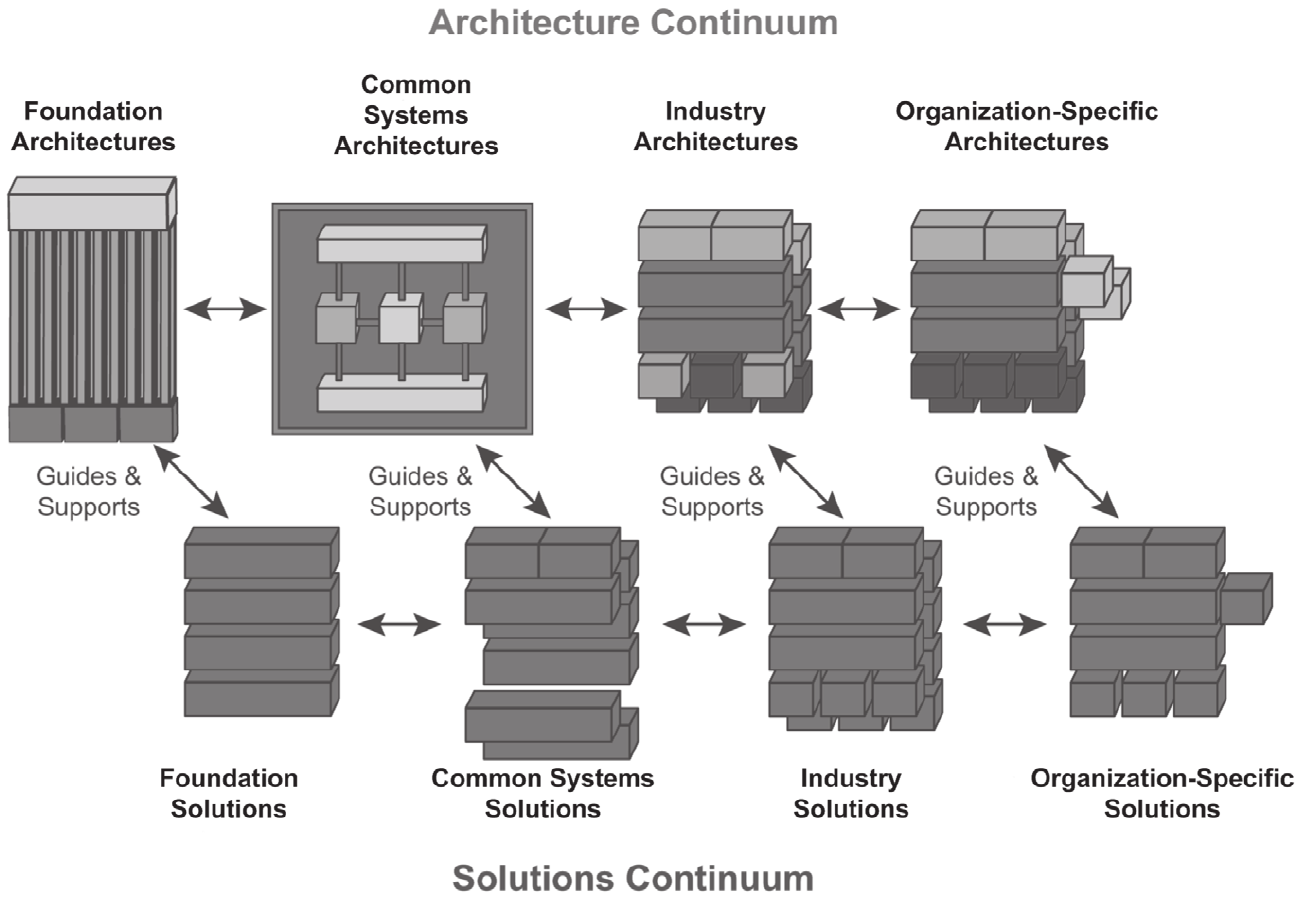
\includegraphics[width=.80\textwidth]{../figures/enterprise_continuum}
            \end{center}
        \end{frame}
    }

    \begin{frame}
        \frametitle{Architecture Repository in TOGAF}
        % \framesubtitle{\hspace{1cm}}
        \vspace{20pt}
        \begin{itemize}
            \item The Architectural Repository is an organized repository for all artifacts produced by an architect during the ADM lifecycle.
            \item This repository helps in the storage, management, and reuse of architectural information.
            \item The architectural landscape in a repository involves three levels: strategic architecture, segment architecture, and capability architecture.
            \item This repository also supports the management and monitoring of Architecture Contracts.
            \item This repository makes it easy to manage artifacts and deliverables in a multi-project environment.
        \end{itemize}
    \end{frame}


    {
        \setbeamertemplate{frametitle}{}
        \setbeamertemplate{navigation symbols}{}
        \setbeamertemplate{footline}{}
        \begin{frame}
            \frametitle{Architecture Repository}
            \framesubtitle{\hspace{1cm}}
            \begin{center}
                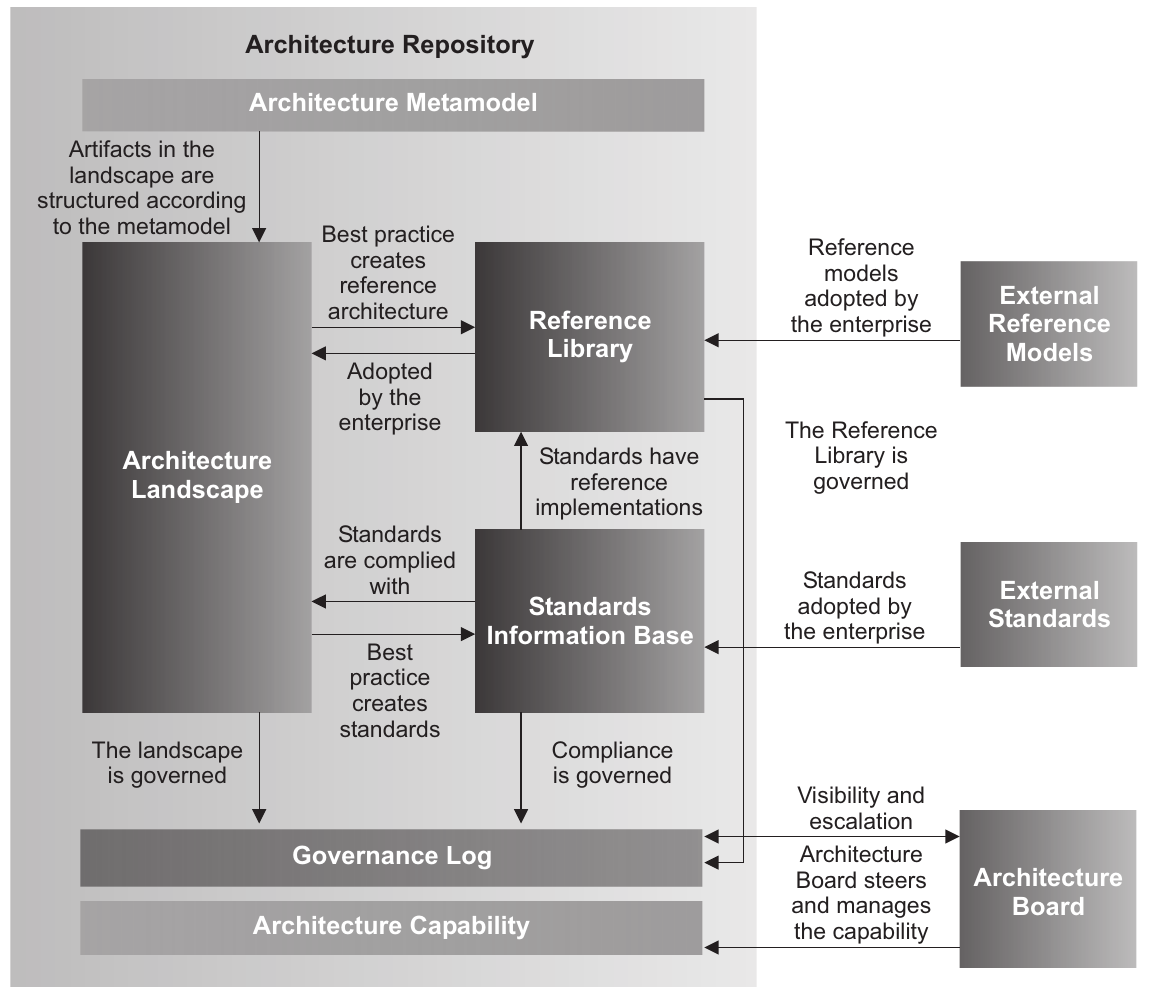
\includegraphics[width=.65\textwidth]{../figures/architecture_repository}
            \end{center}
        \end{frame}
    }




    \begin{frame}
        \frametitle{TOGAF Reference Model}
        % \framesubtitle{\hspace{1cm}}
        \begin{itemize}
            \item The TOGAF Reference Model is a framework that provides a useful starting point for organizations seeking help with their architecture initiatives.
            \item This provides a basic model that can be used as a basis for developing more specific and detailed architectures.
            \item TOGAF Reference Models include the Technical Reference Model (TRM) and the Integrated Information Infrastructure Reference Model (III-RM).

        \end{itemize}
    \end{frame}

    \begin{frame}
        \frametitle{TOGAF Reference Model (2)}
        % \framesubtitle{\hspace{1cm}}
        \begin{itemize}
            \item TRM provides a common model and taxonomy for the technologies that support business applications, such as operating systems, hardware, and networks.
            \item Integrated Information Infrastructure (III-RM) provides a model for architecture and components that enable greater application portability, interoperability, and reuse.
        \end{itemize}
    \end{frame}

    {
        \setbeamertemplate{frametitle}{}
        \setbeamertemplate{navigation symbols}{}
        \setbeamertemplate{footline}{}
        \begin{frame}
            \frametitle{Technical Reference Model}
            \framesubtitle{\hspace{1cm}}
            \begin{center}
                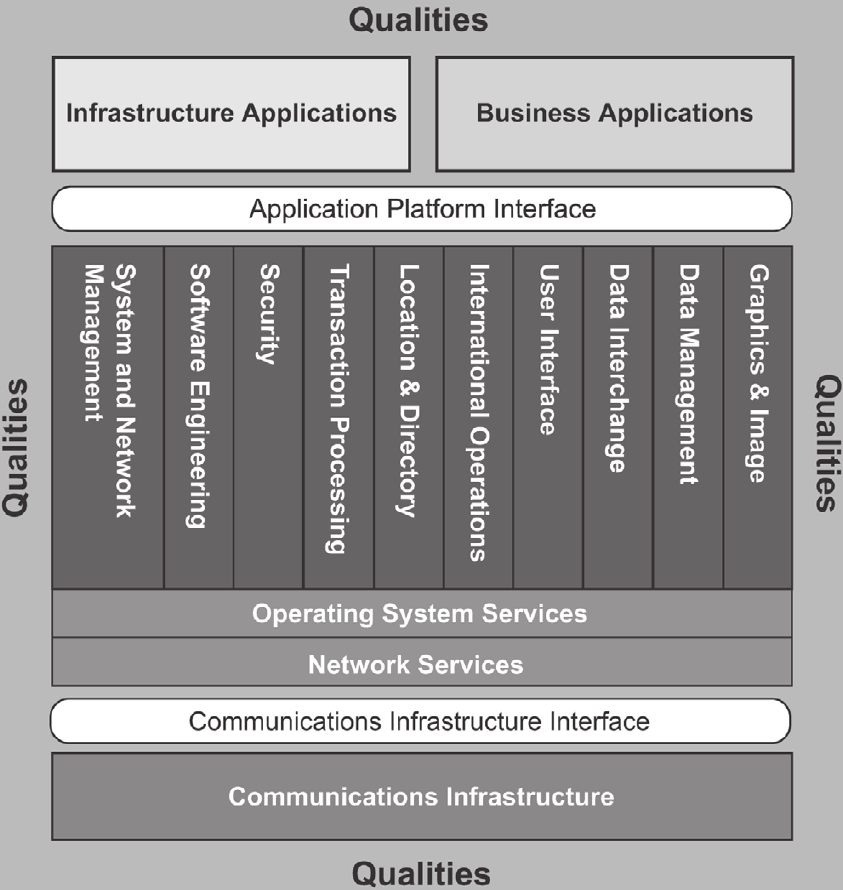
\includegraphics[width=.53\textwidth]{../figures/detailed_technical_reference_model}
            \end{center}
        \end{frame}
    }

    {
        \setbeamertemplate{frametitle}{}
        \setbeamertemplate{navigation symbols}{}
        \setbeamertemplate{footline}{}
        \begin{frame}
            \frametitle{Integrated Information Infrastructure Reference Model}
            \framesubtitle{\hspace{1cm}}
            \begin{center}
                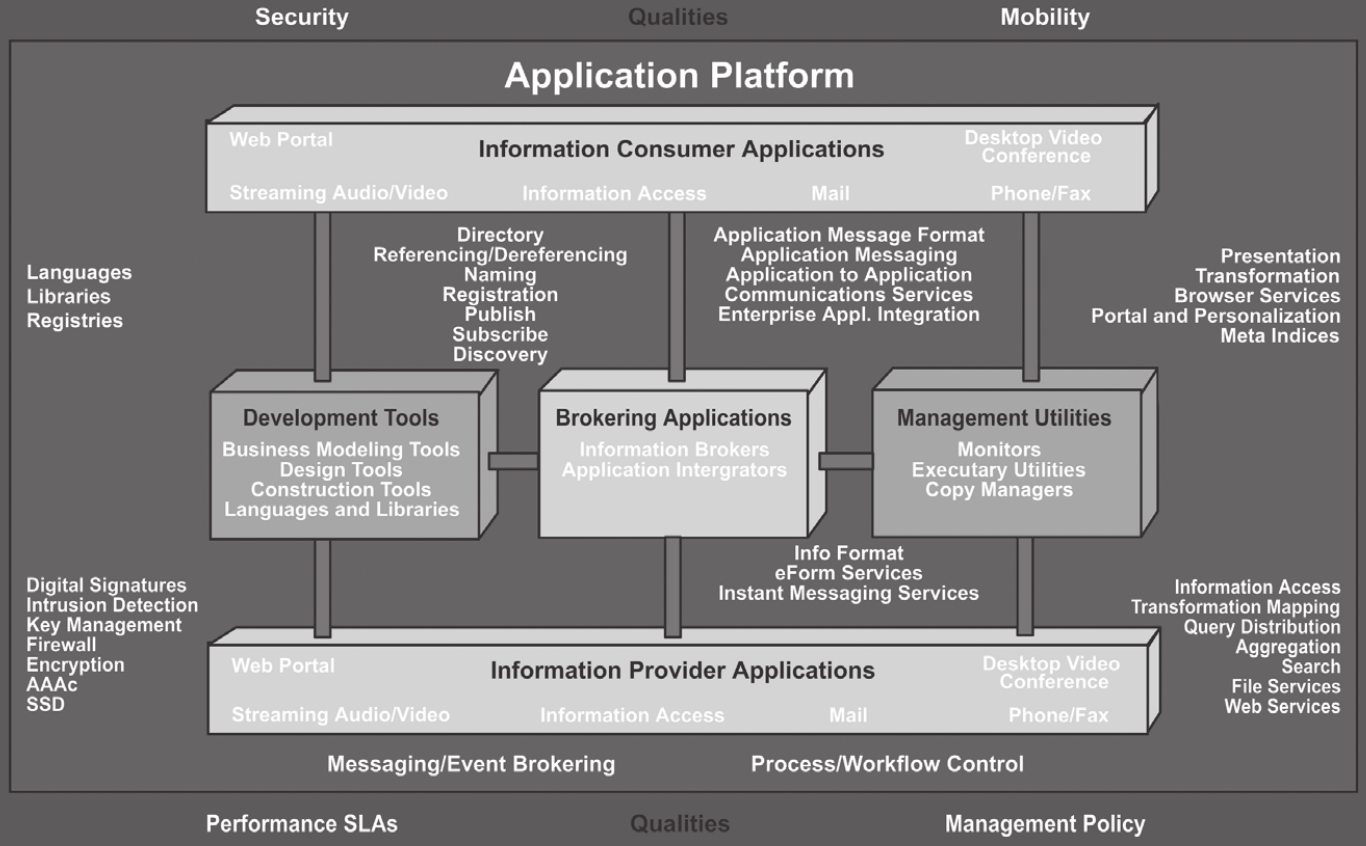
\includegraphics[width=.90\textwidth]{../figures/integrated_information_infrastructure_reference_model}
            \end{center}
        \end{frame}
    }

    \begin{frame}
        \frametitle{Summary}
        % \framesubtitle{\hspace{1cm}}
        \begin{itemize}
            \item TOGAF is a comprehensive enterprise architecture framework that helps organizations design, plan, implement, and manage their information architecture.
            \item TOGAF involves various aspects such as business vision and drivers, business capabilities, capability frameworks, architectural development methods, and others.
            \item In TOGAF, artifacts, deliverables, and building blocks are used to assist in the architecture development process.
        \end{itemize}
    \end{frame}

    \begin{frame}
        \frametitle{Summary (2)}
        % \framesubtitle{\hspace{1cm}}
        \begin{itemize}
            \item The enterprise continuum and tools in TOGAF help organizations understand and utilize this framework effectively.
            \item The TOGAF Architecture Repository and Reference Model is an important knowledge reference component to support the ADM process.
        \end{itemize}
    \end{frame}


\end{document}